\documentclass{article}
\usepackage[utf8]{inputenc}
\usepackage{graphicx}   % Para imágenes.
\usepackage{multicol}
\usepackage{amsmath}
\usepackage{dashrule}
\usepackage{geometry}
\usepackage[spanish, mexico]{babel}
\usepackage{subcaption}
\usepackage[svgnames]{xcolor}
\usepackage{tcolorbox}
\usepackage[table,xcdraw]{xcolor}
\usepackage{fancyhdr}
\usepackage{enumitem}
\usepackage{siunitx}
\usepackage[export]{adjustbox}
\usepackage{multirow}

\definecolor{gray(x11gray)}{rgb}{0.75, 0.75, 0.75}
\definecolor{outerspace}{rgb}{0.25, 0.29, 0.3}
\definecolor{pastelgreen}{rgb}{0.47, 0.87, 0.47}
\definecolor{lincolngreen}{rgb}{0.11, 0.35, 0.02}

\geometry{
    a4paper,
    tmargin = 1.7 cm,
    bmargin = 1.7cm,
    lmargin = 1.5cm,
    rmargin = 1.5cm
}



\pagestyle{fancy}
\fancyhf{}
\cfoot{ \thepage  \hspace{0.5pt}\hspace{0.5pt}}
\lhead{Tarea Examen}

\begin{document}

\thispagestyle{plain}


\hrule
\begin{center}
    {\Large \textbf{UNIVERSIDAD NACIONAL AUTÓNOMA DE MÉXICO}}
    \vspace{10pt}

    {\Large{{Sistemas hibridos en biomedicina}}}
    
    
    \vspace{10pt}

    \hrule

    \vspace{20pt}


    {\Huge \textbf{Tarea 1: Discusión de aritculos sobre tecnicas imagenologicas}}\\
\end{center}

\hdashrule{\linewidth}{1pt}{1mm}

\begin{flushright}
    {\small Medel Garduño Diego} 
\end{flushright}



\section{Imagen de uso diagnostico}


\begin{figure}[h!]
    \centering
    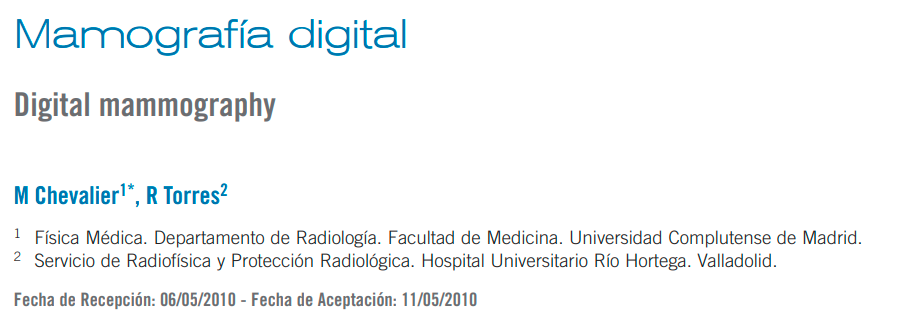
\includegraphics[scale = 0.65]{articulo_mamo.png}
\end{figure}

En principio consideré buscar un articulo en el que la detección por imagen fuera de suma importancia, entonces opte por revisar articulos relacionados con el cancer de mama. Una mastografía al dia de hoy es el estandar de diagnostico preventivo, ya que dada la incidencia de esta patología creciente en la ultima decada, los especialistas buscan la forma de detectar la presencia de cancer antes de que llegue a etapas en avanzadas.

\vspace{10pt} 



El articulo "Digital mammography'' habla de la importancia de la resolucion espacial en las imagenes generados por un mamografo, y es que, retomando lo anteriormente discutido la mamografia es una tecnica que busca prevenir la formación de cancer, ya que se esta observando un aumento en el numero de decesos a nivel mundial. La resolución espacial designa la cantidad minima en unidades de longitud que se pueden apreciar en una imagen de manera nitida, donde con borden bien definidos, entonces mientras mejor resolución espacial posea un instrumento quiere decir que se pueden identificar objetos más pequeños. 

\vspace{10pt}

Un aspecto importante que toca el articulo son las formación de microcalcificaciones,  este tipo de estructuras son las indicadoras de formación de cancer o en el mejor de los casos, son indicio de un tejido tumoral benigno que puede extriparse, por lo que su identificación es de suma importancia, para una biopsia temprana.

\vspace{10pt}


En este articulo se considero un mamografo, aparato que funciona de la misma forma que una radiografía convencional, con la diferencia que utiliza un anodo distinto al tungsteno, ya que el tejido que debe atravesar el haz de rayos x es mucho menor, por ello se consideran anodos de rodio o molibdeno, con rayos x caracteristicos de menor kVp´s. Sin embargo este sistema utiliza un punto focal mucho menor, lo que le permite tener mucha mejor resolución espacial. Sus ventajas son claras en este contexto respecto a la radiografía convencional, en primer lugar la se irradia con menor energía la paciente y en segundo la resolución espacial es tal que se puede identificar tejido milimetrico que represente un riesgo. Si se utilizará la radiografía convencional habrian dos aspectos de precaución, en principio la dosis que recibiría la paciente no estaría justificada, representando un riesgo para ella y en segundo lugar la imagen no tendría ningún uso, ya que sus limitaciones no le permiten identificar las estructuras que se buscan.

\newpage

\section{Imagen en uso terapeutico}

\begin{figure}[h!]
    \centering
    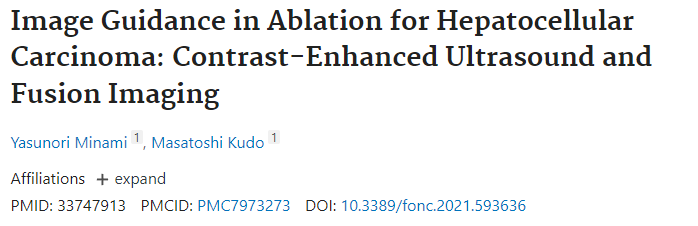
\includegraphics[scale = 0.65]{articulo_CH.png}
\end{figure}


Para este caso consideré el siguiente artículo: `` Image Guidance in Ablation for Hepatocellular Carcinoma: Contrast-Enhanced Ultrasound and Fusion Imaging ''

\vspace{10pt}

El cual en breves palabras muestra como la tecnica de ablación utilizada en el tratamiento de carcinoma hepatocelular mejora al hacer implementar fusión de imagenes de tomográfia axial computarizada o resonancia magnética. En principio la tecnica de ablación es el uso de ondas, como pueden ser microondas o radiofrecuencias con el fin de generar cicatrices en el tejido tumoral, lo que resulta en un control del carcinoma hepatico.
\vspace{10pt}

Previo al tratamiento se suele utilizar sonografía, tecnica imagenologica que hace uso de ondas elasticas (ultrasonido) para la visualización de estructuras, lo anterior permite generar imagenes que sirven para la detección y guia al momento de aplicar el tratamiento. 


\vspace{10pt}

El articulo menciona que en ocasiones el simple hecho de utilizar ultrasonido no basta al momento de identificar donde se encuentra el tumor, para ello se buscaron alternativas. Las más eficaz fue fusionar las imagenes del ultrasonido con las tecnicas de tomografía o de resonancia magnética. Se debe obtener previamente un paquete tridimensional con las tecnicas antes mencionadas, para que al momento del tratamiento estos paquetes de información puedan fusionarse con la imagen actual de ultrasonido, lo que permite tener imagenes con una mayor precisión al momento de designar las fronteras de un tejido tumoral.

\vspace{10pt}

Entonces podemos decir que este articulo hablar de como el sistema de ultrasonido fusionado con tomografia o resonancia magnética permite obtener información valiosa a la hora de aplicar un tramiento de ablación, para asi solo cicatrizar tejido tumoral y no tejido sano. Tanto la tomografia como la resonancia tienen una gran resolución espacial, esa es su principal ventaja, ya que permite distingir los bordes entre estructuras de mejor manera que solo utilizando ultrasonido. 

















\end{document}